En base a los anteriores requisitos el grupo de desarrollo ha generado los siguientes diagramas para el software de la placa de control.

\begin{figure}[H]
    \centering
    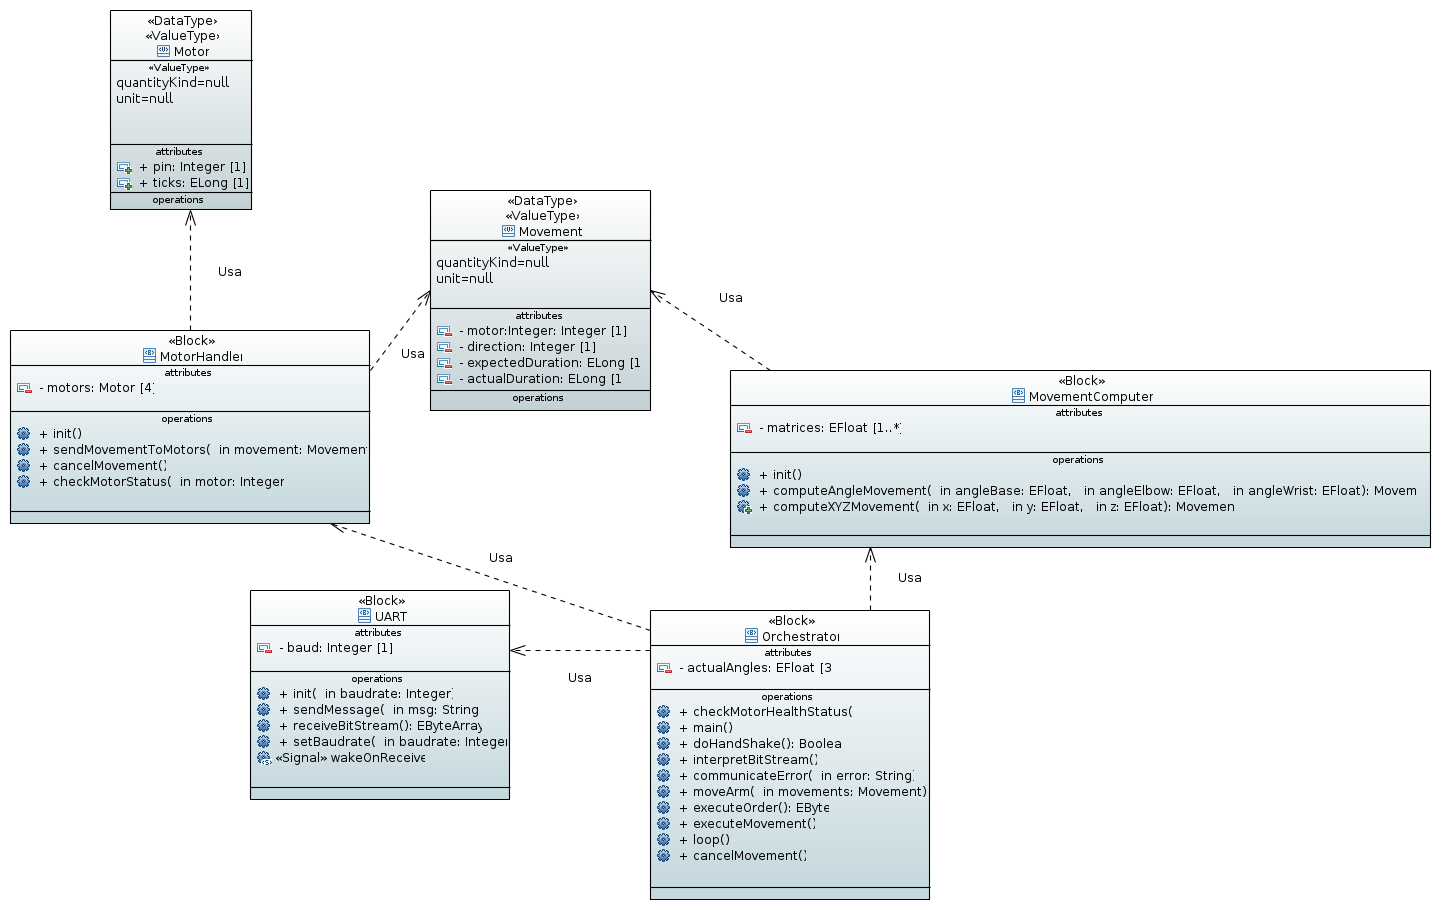
\includegraphics[width=1\linewidth]{pictures/S2BlockDiagram.PNG}
    \caption{Diagrama de bloques del S2}
    \label{fig:diagrama_bloques_s2}
\end{figure}

En el diagrama \ref{fig:diagrama_bloques_s2} se pueden observar los bloques que componen el S2 además de dos tipos de datos los cuales han sido creados para facilitar el control de los motores del brazo.

A continuación se explican cada uno de los bloques:

\begin{itemize}
    \item MotorHandler: Este bloque es capaz de controlar los motores de manera directa empleando el tipo de dato "Movement" enviando la señal necesaria para realizar el movimiento requerido. Además permite verificar el estado de los motores y cancelar los movimientos si esto fuese necesario.
    
    \item UART: Este bloque es el encargado de la comunicación asíncrona entre el S1 y el S2. Controla el ratio de baudios de la comunicación y realiza la transmisión y la recepción de información hasta y desde el S1. A través de este bloque se reciben las ordenes procedentes del S1 y se envían los errores y la posición del brazo al S1 desde el S2.
    
    \item Orchestrator: Encargado de coordinar los demás bloques. En el se encuentra la lógica principal del S2. Algunas de sus funciones mas importantes son interpretar el flujo de bits que llega desde el S1 para obtener una orden concreta; ordenar el movimiento del brazo empleando los demás bloques o hacer el hadshake inicial entre el S1 y el S2. Posteriormente se entrará mas en detalle en el comportamiento de este bloque al analizar los diagramas de estados.
    
    \item MovementComputer: Se encarga de computar el movimiento que se tendrá que comunicar a los motores. Para ello deberá obtener las posiciones deseadas gracias al bloque UART y al Orchestrator.
\end{itemize}

A continuación se explican las dos estructuras de datos que se aprecian en el diagrama \ref{fig:diagrama_bloques_s2}

\begin{itemize}
    \item Motor: Este tipo de dato es empleado por el MotorHandler para saber a que pin debe mandar la señal PWM que gobierna los motores y durante cuantos ticks deberá estar activa dicha señal
    
    \item Movement: El MovementComputer genera un array de 3 posiciones de este tipo de dato, uno por cada motor de giro del brazo. El atributo "motor" guarda un integer que representa uno de los motores del brazo; "direction" sirve para conocer la dirección de giro de dicho motor; "expectedDuration" guarda la duración  
\end{itemize}

A continuación se explican los diagramas de estados de cada uno de los métodos que aparecen en el diagrama de bloques general.

En el caso del Orchestrator tenemos los siguientes diagramas.

\begin{figure}[H]
    \centering
    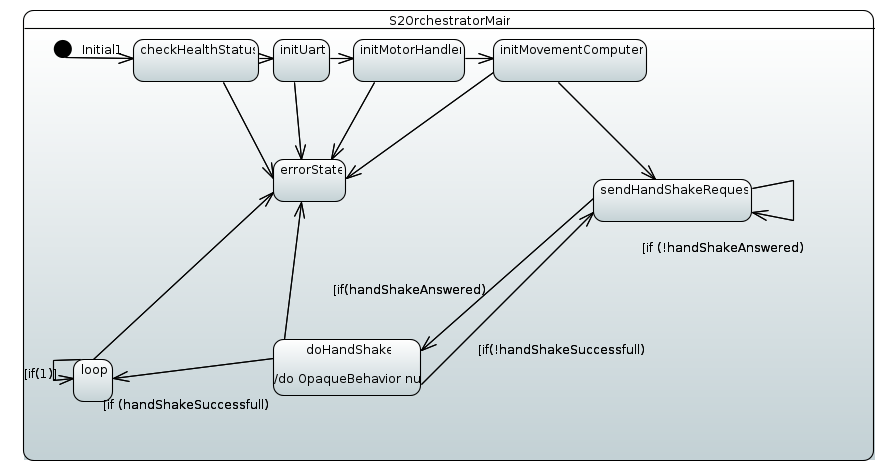
\includegraphics[width=1\linewidth]{pictures/S2OrchestratorMain.PNG}
    \caption{Diagrama de estados del método main() del orchestrator}
    \label{fig:fun_main_orchestrator}
\end{figure}

Este método solo se ejecutará una vez, en cuanto el sistema se ponga en marcha. 

\begin{itemize}
    \item checkHealthStatus: Se verifica la situación de los componentes del brazo robótico para confirmar que todos están en un astado adecuado para el funcionamiento. 
    \item initUart: Se inicializa la UART definiendo un ratio de baudios concreto.
    \item initMotorHandler: Se inicializa el controlador de los motores.
    \item initMovementComputer : Se inicializa el computador de movimientos.
    \item sendHandShakeRequest : Se manda una petición de handshake para verificar si hay algún ordenador conectado. Si se detecta alguno se pasa al siguiente estado, si no, se mantiene en ese estado mandando requests.
    \item doHandShake : Si en el estado anterior se detecta un ordenador se pasa a este estado. Se realiza una serie de intercambios de información para verificar que el ordenador conectado es adecuado para el control del brazo.
    \item loop: Se pasa al bucle de funcionamiento si el handshake ha sido correcto.
    \item errorState: Estado de error al que se llega si en alguno de los estados ocurre algún problema inesperado. 
    
    
\end{itemize}